
% Default to the notebook output style

    


% Inherit from the specified cell style.




    
\documentclass[11pt]{article}

    
    
    \usepackage[T1]{fontenc}
    % Nicer default font (+ math font) than Computer Modern for most use cases
    \usepackage{mathpazo}

    % Basic figure setup, for now with no caption control since it's done
    % automatically by Pandoc (which extracts ![](path) syntax from Markdown).
    \usepackage{graphicx}
    % We will generate all images so they have a width \maxwidth. This means
    % that they will get their normal width if they fit onto the page, but
    % are scaled down if they would overflow the margins.
    \makeatletter
    \def\maxwidth{\ifdim\Gin@nat@width>\linewidth\linewidth
    \else\Gin@nat@width\fi}
    \makeatother
    \let\Oldincludegraphics\includegraphics
    % Set max figure width to be 80% of text width, for now hardcoded.
    \renewcommand{\includegraphics}[1]{\Oldincludegraphics[width=.8\maxwidth]{#1}}
    % Ensure that by default, figures have no caption (until we provide a
    % proper Figure object with a Caption API and a way to capture that
    % in the conversion process - todo).
    \usepackage{caption}
    \DeclareCaptionLabelFormat{nolabel}{}
    \captionsetup{labelformat=nolabel}

    \usepackage{adjustbox} % Used to constrain images to a maximum size 
    \usepackage{xcolor} % Allow colors to be defined
    \usepackage{enumerate} % Needed for markdown enumerations to work
    \usepackage{geometry} % Used to adjust the document margins
    \usepackage{amsmath} % Equations
    \usepackage{amssymb} % Equations
    \usepackage{textcomp} % defines textquotesingle
    % Hack from http://tex.stackexchange.com/a/47451/13684:
    \AtBeginDocument{%
        \def\PYZsq{\textquotesingle}% Upright quotes in Pygmentized code
    }
    \usepackage{upquote} % Upright quotes for verbatim code
    \usepackage{eurosym} % defines \euro
    \usepackage[mathletters]{ucs} % Extended unicode (utf-8) support
    \usepackage[utf8x]{inputenc} % Allow utf-8 characters in the tex document
    \usepackage{fancyvrb} % verbatim replacement that allows latex
    \usepackage{grffile} % extends the file name processing of package graphics 
                         % to support a larger range 
    % The hyperref package gives us a pdf with properly built
    % internal navigation ('pdf bookmarks' for the table of contents,
    % internal cross-reference links, web links for URLs, etc.)
    \usepackage{hyperref}
    \usepackage{longtable} % longtable support required by pandoc >1.10
    \usepackage{booktabs}  % table support for pandoc > 1.12.2
    \usepackage[inline]{enumitem} % IRkernel/repr support (it uses the enumerate* environment)
    \usepackage[normalem]{ulem} % ulem is needed to support strikethroughs (\sout)
                                % normalem makes italics be italics, not underlines
    

    
    
    % Colors for the hyperref package
    \definecolor{urlcolor}{rgb}{0,.145,.698}
    \definecolor{linkcolor}{rgb}{.71,0.21,0.01}
    \definecolor{citecolor}{rgb}{.12,.54,.11}

    % ANSI colors
    \definecolor{ansi-black}{HTML}{3E424D}
    \definecolor{ansi-black-intense}{HTML}{282C36}
    \definecolor{ansi-red}{HTML}{E75C58}
    \definecolor{ansi-red-intense}{HTML}{B22B31}
    \definecolor{ansi-green}{HTML}{00A250}
    \definecolor{ansi-green-intense}{HTML}{007427}
    \definecolor{ansi-yellow}{HTML}{DDB62B}
    \definecolor{ansi-yellow-intense}{HTML}{B27D12}
    \definecolor{ansi-blue}{HTML}{208FFB}
    \definecolor{ansi-blue-intense}{HTML}{0065CA}
    \definecolor{ansi-magenta}{HTML}{D160C4}
    \definecolor{ansi-magenta-intense}{HTML}{A03196}
    \definecolor{ansi-cyan}{HTML}{60C6C8}
    \definecolor{ansi-cyan-intense}{HTML}{258F8F}
    \definecolor{ansi-white}{HTML}{C5C1B4}
    \definecolor{ansi-white-intense}{HTML}{A1A6B2}

    % commands and environments needed by pandoc snippets
    % extracted from the output of `pandoc -s`
    \providecommand{\tightlist}{%
      \setlength{\itemsep}{0pt}\setlength{\parskip}{0pt}}
    \DefineVerbatimEnvironment{Highlighting}{Verbatim}{commandchars=\\\{\}}
    % Add ',fontsize=\small' for more characters per line
    \newenvironment{Shaded}{}{}
    \newcommand{\KeywordTok}[1]{\textcolor[rgb]{0.00,0.44,0.13}{\textbf{{#1}}}}
    \newcommand{\DataTypeTok}[1]{\textcolor[rgb]{0.56,0.13,0.00}{{#1}}}
    \newcommand{\DecValTok}[1]{\textcolor[rgb]{0.25,0.63,0.44}{{#1}}}
    \newcommand{\BaseNTok}[1]{\textcolor[rgb]{0.25,0.63,0.44}{{#1}}}
    \newcommand{\FloatTok}[1]{\textcolor[rgb]{0.25,0.63,0.44}{{#1}}}
    \newcommand{\CharTok}[1]{\textcolor[rgb]{0.25,0.44,0.63}{{#1}}}
    \newcommand{\StringTok}[1]{\textcolor[rgb]{0.25,0.44,0.63}{{#1}}}
    \newcommand{\CommentTok}[1]{\textcolor[rgb]{0.38,0.63,0.69}{\textit{{#1}}}}
    \newcommand{\OtherTok}[1]{\textcolor[rgb]{0.00,0.44,0.13}{{#1}}}
    \newcommand{\AlertTok}[1]{\textcolor[rgb]{1.00,0.00,0.00}{\textbf{{#1}}}}
    \newcommand{\FunctionTok}[1]{\textcolor[rgb]{0.02,0.16,0.49}{{#1}}}
    \newcommand{\RegionMarkerTok}[1]{{#1}}
    \newcommand{\ErrorTok}[1]{\textcolor[rgb]{1.00,0.00,0.00}{\textbf{{#1}}}}
    \newcommand{\NormalTok}[1]{{#1}}
    
    % Additional commands for more recent versions of Pandoc
    \newcommand{\ConstantTok}[1]{\textcolor[rgb]{0.53,0.00,0.00}{{#1}}}
    \newcommand{\SpecialCharTok}[1]{\textcolor[rgb]{0.25,0.44,0.63}{{#1}}}
    \newcommand{\VerbatimStringTok}[1]{\textcolor[rgb]{0.25,0.44,0.63}{{#1}}}
    \newcommand{\SpecialStringTok}[1]{\textcolor[rgb]{0.73,0.40,0.53}{{#1}}}
    \newcommand{\ImportTok}[1]{{#1}}
    \newcommand{\DocumentationTok}[1]{\textcolor[rgb]{0.73,0.13,0.13}{\textit{{#1}}}}
    \newcommand{\AnnotationTok}[1]{\textcolor[rgb]{0.38,0.63,0.69}{\textbf{\textit{{#1}}}}}
    \newcommand{\CommentVarTok}[1]{\textcolor[rgb]{0.38,0.63,0.69}{\textbf{\textit{{#1}}}}}
    \newcommand{\VariableTok}[1]{\textcolor[rgb]{0.10,0.09,0.49}{{#1}}}
    \newcommand{\ControlFlowTok}[1]{\textcolor[rgb]{0.00,0.44,0.13}{\textbf{{#1}}}}
    \newcommand{\OperatorTok}[1]{\textcolor[rgb]{0.40,0.40,0.40}{{#1}}}
    \newcommand{\BuiltInTok}[1]{{#1}}
    \newcommand{\ExtensionTok}[1]{{#1}}
    \newcommand{\PreprocessorTok}[1]{\textcolor[rgb]{0.74,0.48,0.00}{{#1}}}
    \newcommand{\AttributeTok}[1]{\textcolor[rgb]{0.49,0.56,0.16}{{#1}}}
    \newcommand{\InformationTok}[1]{\textcolor[rgb]{0.38,0.63,0.69}{\textbf{\textit{{#1}}}}}
    \newcommand{\WarningTok}[1]{\textcolor[rgb]{0.38,0.63,0.69}{\textbf{\textit{{#1}}}}}
    
    
    % Define a nice break command that doesn't care if a line doesn't already
    % exist.
    \def\br{\hspace*{\fill} \\* }
    % Math Jax compatability definitions
    \def\gt{>}
    \def\lt{<}
    % Document parameters
    \title{Homework 3}
    
    
    

    % Pygments definitions
    
\makeatletter
\def\PY@reset{\let\PY@it=\relax \let\PY@bf=\relax%
    \let\PY@ul=\relax \let\PY@tc=\relax%
    \let\PY@bc=\relax \let\PY@ff=\relax}
\def\PY@tok#1{\csname PY@tok@#1\endcsname}
\def\PY@toks#1+{\ifx\relax#1\empty\else%
    \PY@tok{#1}\expandafter\PY@toks\fi}
\def\PY@do#1{\PY@bc{\PY@tc{\PY@ul{%
    \PY@it{\PY@bf{\PY@ff{#1}}}}}}}
\def\PY#1#2{\PY@reset\PY@toks#1+\relax+\PY@do{#2}}

\expandafter\def\csname PY@tok@w\endcsname{\def\PY@tc##1{\textcolor[rgb]{0.73,0.73,0.73}{##1}}}
\expandafter\def\csname PY@tok@c\endcsname{\let\PY@it=\textit\def\PY@tc##1{\textcolor[rgb]{0.25,0.50,0.50}{##1}}}
\expandafter\def\csname PY@tok@cp\endcsname{\def\PY@tc##1{\textcolor[rgb]{0.74,0.48,0.00}{##1}}}
\expandafter\def\csname PY@tok@k\endcsname{\let\PY@bf=\textbf\def\PY@tc##1{\textcolor[rgb]{0.00,0.50,0.00}{##1}}}
\expandafter\def\csname PY@tok@kp\endcsname{\def\PY@tc##1{\textcolor[rgb]{0.00,0.50,0.00}{##1}}}
\expandafter\def\csname PY@tok@kt\endcsname{\def\PY@tc##1{\textcolor[rgb]{0.69,0.00,0.25}{##1}}}
\expandafter\def\csname PY@tok@o\endcsname{\def\PY@tc##1{\textcolor[rgb]{0.40,0.40,0.40}{##1}}}
\expandafter\def\csname PY@tok@ow\endcsname{\let\PY@bf=\textbf\def\PY@tc##1{\textcolor[rgb]{0.67,0.13,1.00}{##1}}}
\expandafter\def\csname PY@tok@nb\endcsname{\def\PY@tc##1{\textcolor[rgb]{0.00,0.50,0.00}{##1}}}
\expandafter\def\csname PY@tok@nf\endcsname{\def\PY@tc##1{\textcolor[rgb]{0.00,0.00,1.00}{##1}}}
\expandafter\def\csname PY@tok@nc\endcsname{\let\PY@bf=\textbf\def\PY@tc##1{\textcolor[rgb]{0.00,0.00,1.00}{##1}}}
\expandafter\def\csname PY@tok@nn\endcsname{\let\PY@bf=\textbf\def\PY@tc##1{\textcolor[rgb]{0.00,0.00,1.00}{##1}}}
\expandafter\def\csname PY@tok@ne\endcsname{\let\PY@bf=\textbf\def\PY@tc##1{\textcolor[rgb]{0.82,0.25,0.23}{##1}}}
\expandafter\def\csname PY@tok@nv\endcsname{\def\PY@tc##1{\textcolor[rgb]{0.10,0.09,0.49}{##1}}}
\expandafter\def\csname PY@tok@no\endcsname{\def\PY@tc##1{\textcolor[rgb]{0.53,0.00,0.00}{##1}}}
\expandafter\def\csname PY@tok@nl\endcsname{\def\PY@tc##1{\textcolor[rgb]{0.63,0.63,0.00}{##1}}}
\expandafter\def\csname PY@tok@ni\endcsname{\let\PY@bf=\textbf\def\PY@tc##1{\textcolor[rgb]{0.60,0.60,0.60}{##1}}}
\expandafter\def\csname PY@tok@na\endcsname{\def\PY@tc##1{\textcolor[rgb]{0.49,0.56,0.16}{##1}}}
\expandafter\def\csname PY@tok@nt\endcsname{\let\PY@bf=\textbf\def\PY@tc##1{\textcolor[rgb]{0.00,0.50,0.00}{##1}}}
\expandafter\def\csname PY@tok@nd\endcsname{\def\PY@tc##1{\textcolor[rgb]{0.67,0.13,1.00}{##1}}}
\expandafter\def\csname PY@tok@s\endcsname{\def\PY@tc##1{\textcolor[rgb]{0.73,0.13,0.13}{##1}}}
\expandafter\def\csname PY@tok@sd\endcsname{\let\PY@it=\textit\def\PY@tc##1{\textcolor[rgb]{0.73,0.13,0.13}{##1}}}
\expandafter\def\csname PY@tok@si\endcsname{\let\PY@bf=\textbf\def\PY@tc##1{\textcolor[rgb]{0.73,0.40,0.53}{##1}}}
\expandafter\def\csname PY@tok@se\endcsname{\let\PY@bf=\textbf\def\PY@tc##1{\textcolor[rgb]{0.73,0.40,0.13}{##1}}}
\expandafter\def\csname PY@tok@sr\endcsname{\def\PY@tc##1{\textcolor[rgb]{0.73,0.40,0.53}{##1}}}
\expandafter\def\csname PY@tok@ss\endcsname{\def\PY@tc##1{\textcolor[rgb]{0.10,0.09,0.49}{##1}}}
\expandafter\def\csname PY@tok@sx\endcsname{\def\PY@tc##1{\textcolor[rgb]{0.00,0.50,0.00}{##1}}}
\expandafter\def\csname PY@tok@m\endcsname{\def\PY@tc##1{\textcolor[rgb]{0.40,0.40,0.40}{##1}}}
\expandafter\def\csname PY@tok@gh\endcsname{\let\PY@bf=\textbf\def\PY@tc##1{\textcolor[rgb]{0.00,0.00,0.50}{##1}}}
\expandafter\def\csname PY@tok@gu\endcsname{\let\PY@bf=\textbf\def\PY@tc##1{\textcolor[rgb]{0.50,0.00,0.50}{##1}}}
\expandafter\def\csname PY@tok@gd\endcsname{\def\PY@tc##1{\textcolor[rgb]{0.63,0.00,0.00}{##1}}}
\expandafter\def\csname PY@tok@gi\endcsname{\def\PY@tc##1{\textcolor[rgb]{0.00,0.63,0.00}{##1}}}
\expandafter\def\csname PY@tok@gr\endcsname{\def\PY@tc##1{\textcolor[rgb]{1.00,0.00,0.00}{##1}}}
\expandafter\def\csname PY@tok@ge\endcsname{\let\PY@it=\textit}
\expandafter\def\csname PY@tok@gs\endcsname{\let\PY@bf=\textbf}
\expandafter\def\csname PY@tok@gp\endcsname{\let\PY@bf=\textbf\def\PY@tc##1{\textcolor[rgb]{0.00,0.00,0.50}{##1}}}
\expandafter\def\csname PY@tok@go\endcsname{\def\PY@tc##1{\textcolor[rgb]{0.53,0.53,0.53}{##1}}}
\expandafter\def\csname PY@tok@gt\endcsname{\def\PY@tc##1{\textcolor[rgb]{0.00,0.27,0.87}{##1}}}
\expandafter\def\csname PY@tok@err\endcsname{\def\PY@bc##1{\setlength{\fboxsep}{0pt}\fcolorbox[rgb]{1.00,0.00,0.00}{1,1,1}{\strut ##1}}}
\expandafter\def\csname PY@tok@kc\endcsname{\let\PY@bf=\textbf\def\PY@tc##1{\textcolor[rgb]{0.00,0.50,0.00}{##1}}}
\expandafter\def\csname PY@tok@kd\endcsname{\let\PY@bf=\textbf\def\PY@tc##1{\textcolor[rgb]{0.00,0.50,0.00}{##1}}}
\expandafter\def\csname PY@tok@kn\endcsname{\let\PY@bf=\textbf\def\PY@tc##1{\textcolor[rgb]{0.00,0.50,0.00}{##1}}}
\expandafter\def\csname PY@tok@kr\endcsname{\let\PY@bf=\textbf\def\PY@tc##1{\textcolor[rgb]{0.00,0.50,0.00}{##1}}}
\expandafter\def\csname PY@tok@bp\endcsname{\def\PY@tc##1{\textcolor[rgb]{0.00,0.50,0.00}{##1}}}
\expandafter\def\csname PY@tok@fm\endcsname{\def\PY@tc##1{\textcolor[rgb]{0.00,0.00,1.00}{##1}}}
\expandafter\def\csname PY@tok@vc\endcsname{\def\PY@tc##1{\textcolor[rgb]{0.10,0.09,0.49}{##1}}}
\expandafter\def\csname PY@tok@vg\endcsname{\def\PY@tc##1{\textcolor[rgb]{0.10,0.09,0.49}{##1}}}
\expandafter\def\csname PY@tok@vi\endcsname{\def\PY@tc##1{\textcolor[rgb]{0.10,0.09,0.49}{##1}}}
\expandafter\def\csname PY@tok@vm\endcsname{\def\PY@tc##1{\textcolor[rgb]{0.10,0.09,0.49}{##1}}}
\expandafter\def\csname PY@tok@sa\endcsname{\def\PY@tc##1{\textcolor[rgb]{0.73,0.13,0.13}{##1}}}
\expandafter\def\csname PY@tok@sb\endcsname{\def\PY@tc##1{\textcolor[rgb]{0.73,0.13,0.13}{##1}}}
\expandafter\def\csname PY@tok@sc\endcsname{\def\PY@tc##1{\textcolor[rgb]{0.73,0.13,0.13}{##1}}}
\expandafter\def\csname PY@tok@dl\endcsname{\def\PY@tc##1{\textcolor[rgb]{0.73,0.13,0.13}{##1}}}
\expandafter\def\csname PY@tok@s2\endcsname{\def\PY@tc##1{\textcolor[rgb]{0.73,0.13,0.13}{##1}}}
\expandafter\def\csname PY@tok@sh\endcsname{\def\PY@tc##1{\textcolor[rgb]{0.73,0.13,0.13}{##1}}}
\expandafter\def\csname PY@tok@s1\endcsname{\def\PY@tc##1{\textcolor[rgb]{0.73,0.13,0.13}{##1}}}
\expandafter\def\csname PY@tok@mb\endcsname{\def\PY@tc##1{\textcolor[rgb]{0.40,0.40,0.40}{##1}}}
\expandafter\def\csname PY@tok@mf\endcsname{\def\PY@tc##1{\textcolor[rgb]{0.40,0.40,0.40}{##1}}}
\expandafter\def\csname PY@tok@mh\endcsname{\def\PY@tc##1{\textcolor[rgb]{0.40,0.40,0.40}{##1}}}
\expandafter\def\csname PY@tok@mi\endcsname{\def\PY@tc##1{\textcolor[rgb]{0.40,0.40,0.40}{##1}}}
\expandafter\def\csname PY@tok@il\endcsname{\def\PY@tc##1{\textcolor[rgb]{0.40,0.40,0.40}{##1}}}
\expandafter\def\csname PY@tok@mo\endcsname{\def\PY@tc##1{\textcolor[rgb]{0.40,0.40,0.40}{##1}}}
\expandafter\def\csname PY@tok@ch\endcsname{\let\PY@it=\textit\def\PY@tc##1{\textcolor[rgb]{0.25,0.50,0.50}{##1}}}
\expandafter\def\csname PY@tok@cm\endcsname{\let\PY@it=\textit\def\PY@tc##1{\textcolor[rgb]{0.25,0.50,0.50}{##1}}}
\expandafter\def\csname PY@tok@cpf\endcsname{\let\PY@it=\textit\def\PY@tc##1{\textcolor[rgb]{0.25,0.50,0.50}{##1}}}
\expandafter\def\csname PY@tok@c1\endcsname{\let\PY@it=\textit\def\PY@tc##1{\textcolor[rgb]{0.25,0.50,0.50}{##1}}}
\expandafter\def\csname PY@tok@cs\endcsname{\let\PY@it=\textit\def\PY@tc##1{\textcolor[rgb]{0.25,0.50,0.50}{##1}}}

\def\PYZbs{\char`\\}
\def\PYZus{\char`\_}
\def\PYZob{\char`\{}
\def\PYZcb{\char`\}}
\def\PYZca{\char`\^}
\def\PYZam{\char`\&}
\def\PYZlt{\char`\<}
\def\PYZgt{\char`\>}
\def\PYZsh{\char`\#}
\def\PYZpc{\char`\%}
\def\PYZdl{\char`\$}
\def\PYZhy{\char`\-}
\def\PYZsq{\char`\'}
\def\PYZdq{\char`\"}
\def\PYZti{\char`\~}
% for compatibility with earlier versions
\def\PYZat{@}
\def\PYZlb{[}
\def\PYZrb{]}
\makeatother


    % Exact colors from NB
    \definecolor{incolor}{rgb}{0.0, 0.0, 0.5}
    \definecolor{outcolor}{rgb}{0.545, 0.0, 0.0}



    
    % Prevent overflowing lines due to hard-to-break entities
    \sloppy 
    % Setup hyperref package
    \hypersetup{
      breaklinks=true,  % so long urls are correctly broken across lines
      colorlinks=true,
      urlcolor=urlcolor,
      linkcolor=linkcolor,
      citecolor=citecolor,
      }
    % Slightly bigger margins than the latex defaults
    
    \geometry{verbose,tmargin=1in,bmargin=1in,lmargin=1in,rmargin=1in}
    
    

    \begin{document}    

    
    \section*{IE6511 Homework 3}\label{ie6511-homework-3}

Done by: Aloisius Stephen and Yang Xiaozhou

    \begin{Verbatim}[commandchars=\\\{\}]
{\color{incolor}In [{\color{incolor}14}]:} \PY{k+kn}{import} \PY{n+nn}{numpy} \PY{k}{as} \PY{n+nn}{np}
         \PY{k+kn}{import} \PY{n+nn}{pandas} \PY{k}{as} \PY{n+nn}{pd}
         \PY{k+kn}{import} \PY{n+nn}{matplotlib}
         \PY{k+kn}{import} \PY{n+nn}{matplotlib}\PY{n+nn}{.}\PY{n+nn}{pyplot} \PY{k}{as} \PY{n+nn}{plt}
         \PY{o}{\PYZpc{}}\PY{k}{matplotlib} inline
         
         \PY{n}{np}\PY{o}{.}\PY{n}{set\PYZus{}printoptions}\PY{p}{(}\PY{n}{precision}\PY{o}{=}\PY{l+m+mi}{3}\PY{p}{)}
         
         \PY{n}{font} \PY{o}{=} \PY{p}{\PYZob{}}\PY{l+s+s1}{\PYZsq{}}\PY{l+s+s1}{family}\PY{l+s+s1}{\PYZsq{}} \PY{p}{:} \PY{l+s+s1}{\PYZsq{}}\PY{l+s+s1}{sans\PYZhy{}serif}\PY{l+s+s1}{\PYZsq{}}\PY{p}{,}
                 \PY{l+s+s1}{\PYZsq{}}\PY{l+s+s1}{weight}\PY{l+s+s1}{\PYZsq{}} \PY{p}{:} \PY{l+s+s1}{\PYZsq{}}\PY{l+s+s1}{normal}\PY{l+s+s1}{\PYZsq{}}\PY{p}{,}
                 \PY{l+s+s1}{\PYZsq{}}\PY{l+s+s1}{size}\PY{l+s+s1}{\PYZsq{}}   \PY{p}{:} \PY{l+m+mi}{12}\PY{p}{\PYZcb{}}
         
         \PY{n}{matplotlib}\PY{o}{.}\PY{n}{rc}\PY{p}{(}\PY{l+s+s1}{\PYZsq{}}\PY{l+s+s1}{font}\PY{l+s+s1}{\PYZsq{}}\PY{p}{,} \PY{o}{*}\PY{o}{*}\PY{n}{font}\PY{p}{)}
\end{Verbatim}


    \subsection*{Question 1. Markov Chain Configuration Graph with Random
Walk}\label{question-1.-markov-chain-configuration-graph-with-random-walk}

\begin{enumerate}
\def\labelenumi{\alph{enumi})}
\item
  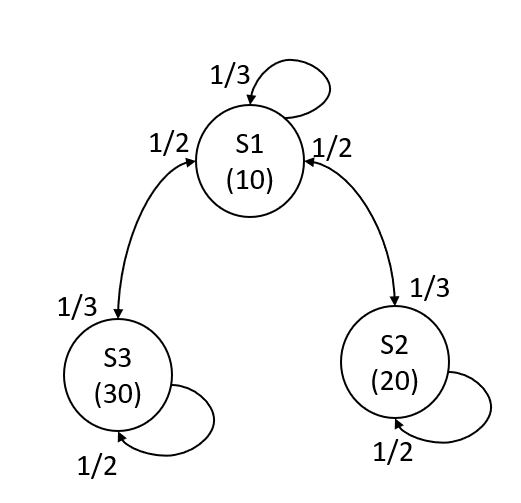
\includegraphics{1a} 
  \medbreak
\item
  transition probability matrix

  \begin{align*}
  \Theta &= 
  \begin{bmatrix}
  \frac{1}{3} & \frac{1}{3} & \frac{1}{3} \\
  \frac{1}{2} & \frac{1}{2} & 0 \\
  \frac{1}{2} & 0 & \frac{1}{2}
  \end{bmatrix}
  \end{align*}
  \bigbreak
\item
  convergence probability matrix Let \(\pi = [ a \quad b \quad b ]\)
  where \(a,b \in [0,1]\) and \(a+b+b=1\), 
\end{enumerate}

\begin{align*}
\pi &= \pi \Theta\\
\begin{bmatrix}
a & b & b \\
\end{bmatrix}
&=
\begin{bmatrix}
a & b & b \\
\end{bmatrix}
\begin{bmatrix}
\frac{1}{3} & \frac{1}{3} & \frac{1}{3} \\
\frac{1}{2} & \frac{1}{2} & 0 \\
\frac{1}{2} & 0 & \frac{1}{2}
\end{bmatrix} \\
&\Rightarrow \frac{1}{3}a + \frac{1}{2}b + \frac{1}{2}b = a\\
&\Rightarrow b = \frac{2}{3}a \\
\end{align*}

Substituting to
\(a+b+b=1 \Rightarrow a+\frac{2}{3}a+\frac{2}{3}a = 1 \Rightarrow a = \frac{3}{7}\)

 Therefore solving for \(b = \frac{2}{3}a = \frac{2}{7}\), we get

\begin{align*}
\pi &= 
\begin{bmatrix}
\frac{3}{7} & \frac{2}{7} & \frac{2}{7} \\
\end{bmatrix}
\end{align*}

The values of \(\pi_2,\pi_3\) are equal because the random walk from S2
and S3 are similar, such that they can only go to either S1 or stay
where they are with probability of 0.5. As for \(\pi_1\) being slightly
larger than the other two convergence probability, it is because from
node S2 and S3 they can only go to S1 with probability of 1/2, however
from S1 it can go to S2 or S3 with probability of 1/3.

    \subsection*{Question 2. Theory-Configuration Graph and transition
probability
matrix-Greedy}\label{question-2.-theory-configuration-graph-and-transition-probability-matrix-greedy}

\begin{enumerate}
\def\labelenumi{\alph{enumi})}
\tightlist
\item
  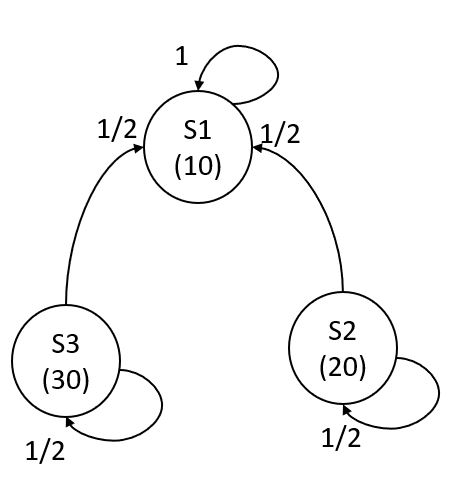
\includegraphics{2a} 
\end{enumerate}
\medbreak 
b)Transition probability matrix

\begin{align*}
\Theta &= 
\begin{bmatrix}
1 & 0 & 0 \\
\frac{1}{2} & \frac{1}{2} & 0 \\
\frac{1}{2} & 0 & \frac{1}{2}
\end{bmatrix}
\end{align*}

\begin{enumerate}
\def\labelenumi{\alph{enumi})}
\setcounter{enumi}{2}
\tightlist
\item
  Convergence Probability Matrix

  \begin{align*}
  \pi &= 
  \begin{bmatrix}
  1& 0 & 0 \\
  \end{bmatrix}
  \end{align*}
\end{enumerate}

check:

\begin{align*}
\pi \Theta &=
\begin{bmatrix}
1 & 0 & 0 \\
\end{bmatrix}
\begin{bmatrix}
1 & 0 & 0 \\
\frac{1}{2} & \frac{1}{2} & 0 \\
\frac{1}{2} & 0 & \frac{1}{2}
\end{bmatrix} 
= 
\begin{bmatrix}
1 & 0 & 0 \\
\end{bmatrix}\\
&= \pi \\
\end{align*}

The values of \(\pi_2,\pi_3\) are equal to 0 because once the search
moves out of S2 and S3 to S1, it will remain in S1 since there are no
better solution, which is why \(\pi_1 =1\) 

    \subsection*{Question 3. Configuration SA Transition and convergence
Theory}\label{question-3.-configuration-sa-transition-and-convergence-theory}

    \begin{enumerate}
\def\labelenumi{\alph{enumi})}
\tightlist
\item
  Cost for each state:
\end{enumerate}

    \begin{Verbatim}[commandchars=\\\{\}]
{\color{incolor}In [{\color{incolor}15}]:} \PY{k}{def} \PY{n+nf}{cost}\PY{p}{(}\PY{n}{x1}\PY{p}{,}\PY{n}{x2}\PY{p}{)}\PY{p}{:}
             \PY{k}{return} \PY{l+m+mi}{2}\PY{o}{*}\PY{n}{np}\PY{o}{.}\PY{n}{power}\PY{p}{(}\PY{p}{(}\PY{n}{x1}\PY{o}{\PYZhy{}}\PY{n}{x2}\PY{p}{)}\PY{p}{,}\PY{l+m+mi}{2}\PY{p}{)} \PY{o}{+} \PY{n}{x1}
         
         \PY{n+nb}{print}\PY{p}{(}\PY{l+s+s2}{\PYZdq{}}\PY{l+s+s2}{State1=(0,1) Costs= }\PY{l+s+si}{\PYZpc{}.4f}\PY{l+s+s2}{\PYZdq{}} \PY{o}{\PYZpc{}}\PY{k}{cost}(0,1))
         \PY{n+nb}{print}\PY{p}{(}\PY{l+s+s2}{\PYZdq{}}\PY{l+s+s2}{State2=(1,1) Costs= }\PY{l+s+si}{\PYZpc{}.4f}\PY{l+s+s2}{\PYZdq{}} \PY{o}{\PYZpc{}}\PY{k}{cost}(1,1))
         \PY{n+nb}{print}\PY{p}{(}\PY{l+s+s2}{\PYZdq{}}\PY{l+s+s2}{State3=(0,0) Costs= }\PY{l+s+si}{\PYZpc{}.4f}\PY{l+s+s2}{\PYZdq{}} \PY{o}{\PYZpc{}}\PY{k}{cost}(0,0))
         \PY{n+nb}{print}\PY{p}{(}\PY{l+s+s2}{\PYZdq{}}\PY{l+s+s2}{State4=(1,0) Costs= }\PY{l+s+si}{\PYZpc{}.4f}\PY{l+s+s2}{\PYZdq{}} \PY{o}{\PYZpc{}}\PY{k}{cost}(1,0))
\end{Verbatim}


    \begin{Verbatim}[commandchars=\\\{\}]
State1=(0,1) Costs= 2.0000
State2=(1,1) Costs= 1.0000
State3=(0,0) Costs= 0.0000
State4=(1,0) Costs= 3.0000

    \end{Verbatim}

    Transition probability

\begin{align*}
P_{12} &=  P_{13} = \frac{1}{2} \\
P_{21} &= 0.5 e^\frac{-1}{T}, \quad P_{24}= 0.5 e^\frac{-2}{T}\\
P_{22} &= 1-0.5 e^\frac{-1}{T} -0.5 e^\frac{-2}{T}\\
P_{31} &= 0.5 e^\frac{-2}{T}, \quad P_{34} = 0.5 e^\frac{-3}{T}\\
P_{33} &= 1-0.5 e^\frac{-2}{T}-0.5 e^\frac{-3}{T}\\
P_{42} &= P_{43} = \frac{1}{2} \\
\end{align*}

There are no self-loops for states 1 and 4 because its neighbours have
lower costs in both cases therefore the state will move to either 2 or
3, and not stay at its original state as there is no potential uphill
move that can be rejected.
\medbreak
    b)Transition probability matrix For \(T = 1\),

    \begin{Verbatim}[commandchars=\\\{\}]
{\color{incolor}In [{\color{incolor}16}]:} \PY{k}{def} \PY{n+nf}{transProb}\PY{p}{(}\PY{n}{T}\PY{p}{)}\PY{p}{:}
         
             \PY{n}{p21} \PY{o}{=} \PY{l+m+mf}{0.5}\PY{o}{*}\PY{n}{np}\PY{o}{.}\PY{n}{exp}\PY{p}{(}\PY{o}{\PYZhy{}}\PY{l+m+mi}{1}\PY{o}{/}\PY{n}{T}\PY{p}{)}
             \PY{n}{p24} \PY{o}{=} \PY{l+m+mf}{0.5}\PY{o}{*}\PY{n}{np}\PY{o}{.}\PY{n}{exp}\PY{p}{(}\PY{o}{\PYZhy{}}\PY{l+m+mi}{2}\PY{o}{/}\PY{n}{T}\PY{p}{)}
             \PY{n}{p22} \PY{o}{=} \PY{l+m+mi}{1}\PY{o}{\PYZhy{}}\PY{n}{p21}\PY{o}{\PYZhy{}}\PY{n}{p24}
         
             \PY{n+nb}{print}\PY{p}{(}\PY{l+s+s2}{\PYZdq{}}\PY{l+s+s2}{P\PYZus{}21 = }\PY{l+s+si}{\PYZpc{}.6f}\PY{l+s+s2}{\PYZdq{}} \PY{o}{\PYZpc{}}\PY{k}{p21})
             \PY{n+nb}{print}\PY{p}{(}\PY{l+s+s2}{\PYZdq{}}\PY{l+s+s2}{P\PYZus{}24 = }\PY{l+s+si}{\PYZpc{}.6f}\PY{l+s+s2}{\PYZdq{}} \PY{o}{\PYZpc{}}\PY{k}{p24})
             \PY{n+nb}{print}\PY{p}{(}\PY{l+s+s2}{\PYZdq{}}\PY{l+s+s2}{P\PYZus{}22 = }\PY{l+s+si}{\PYZpc{}.6f}\PY{l+s+s2}{\PYZdq{}} \PY{o}{\PYZpc{}}\PY{k}{p22})
         
             \PY{n}{p31} \PY{o}{=} \PY{l+m+mf}{0.5}\PY{o}{*}\PY{n}{np}\PY{o}{.}\PY{n}{exp}\PY{p}{(}\PY{o}{\PYZhy{}}\PY{l+m+mi}{2}\PY{o}{/}\PY{n}{T}\PY{p}{)}
             \PY{n}{p34} \PY{o}{=} \PY{l+m+mf}{0.5}\PY{o}{*}\PY{n}{np}\PY{o}{.}\PY{n}{exp}\PY{p}{(}\PY{o}{\PYZhy{}}\PY{l+m+mi}{3}\PY{o}{/}\PY{n}{T}\PY{p}{)}
             \PY{n}{p33} \PY{o}{=} \PY{l+m+mi}{1}\PY{o}{\PYZhy{}}\PY{n}{p31}\PY{o}{\PYZhy{}}\PY{n}{p34}
             
             \PY{n+nb}{print}\PY{p}{(}\PY{l+s+s2}{\PYZdq{}}\PY{l+s+se}{\PYZbs{}n}\PY{l+s+s2}{P\PYZus{}31 = }\PY{l+s+si}{\PYZpc{}.6f}\PY{l+s+s2}{\PYZdq{}} \PY{o}{\PYZpc{}}\PY{k}{p31})
             \PY{n+nb}{print}\PY{p}{(}\PY{l+s+s2}{\PYZdq{}}\PY{l+s+s2}{P\PYZus{}34 = }\PY{l+s+si}{\PYZpc{}.6f}\PY{l+s+s2}{\PYZdq{}} \PY{o}{\PYZpc{}}\PY{k}{p34})
             \PY{n+nb}{print}\PY{p}{(}\PY{l+s+s2}{\PYZdq{}}\PY{l+s+s2}{P\PYZus{}33 = }\PY{l+s+si}{\PYZpc{}.6f}\PY{l+s+s2}{\PYZdq{}} \PY{o}{\PYZpc{}}\PY{k}{p33})
             
             \PY{n}{P} \PY{o}{=} \PY{n}{np}\PY{o}{.}\PY{n}{matrix}\PY{p}{(}\PY{p}{[}\PY{p}{[}\PY{l+m+mi}{0}\PY{p}{,}\PY{l+m+mf}{0.5}\PY{p}{,}\PY{l+m+mf}{0.5}\PY{p}{,}\PY{l+m+mi}{0}\PY{p}{]}\PY{p}{,}\PY{p}{[}\PY{n}{p21}\PY{p}{,}\PY{n}{p22}\PY{p}{,}\PY{l+m+mi}{0}\PY{p}{,}\PY{n}{p24}\PY{p}{]}\PY{p}{,}\PY{p}{[}\PY{n}{p31}\PY{p}{,}\PY{l+m+mi}{0}\PY{p}{,}\PY{n}{p33}\PY{p}{,}\PY{n}{p34}\PY{p}{]}\PY{p}{,}\PY{p}{[}\PY{l+m+mi}{0}\PY{p}{,}\PY{l+m+mf}{0.5}\PY{p}{,}\PY{l+m+mf}{0.5}\PY{p}{,}\PY{l+m+mi}{0}\PY{p}{]}\PY{p}{]}\PY{p}{)}
             \PY{n+nb}{print}\PY{p}{(}\PY{l+s+s2}{\PYZdq{}}\PY{l+s+se}{\PYZbs{}n}\PY{l+s+s2}{P = }\PY{l+s+s2}{\PYZdq{}}\PY{p}{)}
             \PY{n+nb}{print}\PY{p}{(}\PY{n}{P}\PY{p}{)}
             \PY{k}{return} \PY{n}{P}
         
         \PY{n}{P} \PY{o}{=} \PY{n}{transProb}\PY{p}{(}\PY{l+m+mi}{1}\PY{p}{)}
\end{Verbatim}


    \begin{Verbatim}[commandchars=\\\{\}]
P\_21 = 0.183940
P\_24 = 0.067668
P\_22 = 0.748393

P\_31 = 0.067668
P\_34 = 0.024894
P\_33 = 0.907439

P = 
[[ 0.     0.5    0.5    0.   ]
 [ 0.184  0.748  0.     0.068]
 [ 0.068  0.     0.907  0.025]
 [ 0.     0.5    0.5    0.   ]]

    \end{Verbatim}

    \begin{enumerate}
\def\labelenumi{\alph{enumi})}
\setcounter{enumi}{2}

\newpage
\item
\end{enumerate}

    \begin{Verbatim}[commandchars=\\\{\}]
{\color{incolor}In [{\color{incolor}17}]:} \PY{k}{def} \PY{n+nf}{matPower}\PY{p}{(}\PY{n}{matrix}\PY{p}{,}\PY{n}{power}\PY{p}{)}\PY{p}{:}
             \PY{n}{sol} \PY{o}{=} \PY{n}{matrix}
         
             \PY{k}{for} \PY{n}{i} \PY{o+ow}{in} \PY{n+nb}{range}\PY{p}{(}\PY{l+m+mi}{1}\PY{p}{,}\PY{n}{power}\PY{p}{)}\PY{p}{:}
                 \PY{n}{sol} \PY{o}{=} \PY{n}{np}\PY{o}{.}\PY{n}{matmul}\PY{p}{(}\PY{n}{sol}\PY{p}{,}\PY{n}{matrix}\PY{p}{)}
             
             \PY{k}{return} \PY{n}{sol}
         
         \PY{n}{P\PYZus{}5} \PY{o}{=} \PY{n}{matPower}\PY{p}{(}\PY{n}{P}\PY{p}{,}\PY{l+m+mi}{5}\PY{p}{)}
         \PY{n}{P\PYZus{}10} \PY{o}{=} \PY{n}{matPower}\PY{p}{(}\PY{n}{P}\PY{p}{,}\PY{l+m+mi}{10}\PY{p}{)}
         \PY{n}{P\PYZus{}1000} \PY{o}{=} \PY{n}{matPower}\PY{p}{(}\PY{n}{P}\PY{p}{,}\PY{l+m+mi}{1000}\PY{p}{)}
         
         \PY{n+nb}{print}\PY{p}{(}\PY{l+s+s2}{\PYZdq{}}\PY{l+s+se}{\PYZbs{}n}\PY{l+s+s2}{P\PYZca{}5=}\PY{l+s+s2}{\PYZdq{}}\PY{p}{)}
         \PY{n+nb}{print}\PY{p}{(}\PY{n}{P\PYZus{}5}\PY{p}{)}
         \PY{n+nb}{print}\PY{p}{(}\PY{l+s+s2}{\PYZdq{}}\PY{l+s+s2}{P\PYZca{}10=}\PY{l+s+s2}{\PYZdq{}}\PY{p}{)}
         \PY{n+nb}{print}\PY{p}{(}\PY{n}{P\PYZus{}10}\PY{p}{)}
         \PY{n+nb}{print}\PY{p}{(}\PY{l+s+s2}{\PYZdq{}}\PY{l+s+s2}{P\PYZca{}1000=}\PY{l+s+s2}{\PYZdq{}}\PY{p}{)}
         \PY{n+nb}{print}\PY{p}{(}\PY{n}{P\PYZus{}1000}\PY{p}{)}
\end{Verbatim}


    \begin{Verbatim}[commandchars=\\\{\}]

P\^{}5=
[[ 0.098  0.325  0.541  0.036]
 [ 0.12   0.495  0.341  0.044]
 [ 0.073  0.126  0.774  0.027]
 [ 0.098  0.325  0.541  0.036]]
P\^{}10=
[[ 0.092  0.272  0.602  0.034]
 [ 0.1    0.341  0.522  0.037]
 [ 0.082  0.192  0.697  0.03 ]
 [ 0.092  0.272  0.602  0.034]]
P\^{}1000=
[[ 0.087  0.237  0.644  0.032]
 [ 0.087  0.237  0.644  0.032]
 [ 0.087  0.237  0.644  0.032]
 [ 0.087  0.237  0.644  0.032]]

    \end{Verbatim}

    The probability distribution will be
\(\,[0.087 \quad 0.237 \quad 0.644 \quad 0.032]\)

    \begin{enumerate}
\def\labelenumi{\alph{enumi})}
\setcounter{enumi}{3}
\tightlist
\newpage
\item
  for T= 10
\end{enumerate}

    \begin{Verbatim}[commandchars=\\\{\}]
{\color{incolor}In [{\color{incolor}18}]:} \PY{n}{P} \PY{o}{=} \PY{n}{transProb}\PY{p}{(}\PY{l+m+mi}{10}\PY{p}{)}
         \PY{n}{P\PYZus{}5} \PY{o}{=} \PY{n}{matPower}\PY{p}{(}\PY{n}{P}\PY{p}{,}\PY{l+m+mi}{5}\PY{p}{)}
         \PY{n}{P\PYZus{}10} \PY{o}{=} \PY{n}{matPower}\PY{p}{(}\PY{n}{P}\PY{p}{,}\PY{l+m+mi}{10}\PY{p}{)}
         \PY{n}{P\PYZus{}1000} \PY{o}{=} \PY{n}{matPower}\PY{p}{(}\PY{n}{P}\PY{p}{,}\PY{l+m+mi}{1000}\PY{p}{)}
         
         \PY{n+nb}{print}\PY{p}{(}\PY{l+s+s2}{\PYZdq{}}\PY{l+s+se}{\PYZbs{}n}\PY{l+s+s2}{P\PYZca{}5=}\PY{l+s+s2}{\PYZdq{}}\PY{p}{)}
         \PY{n+nb}{print}\PY{p}{(}\PY{n}{P\PYZus{}5}\PY{p}{)}
         \PY{n+nb}{print}\PY{p}{(}\PY{l+s+s2}{\PYZdq{}}\PY{l+s+s2}{P\PYZca{}10=}\PY{l+s+s2}{\PYZdq{}}\PY{p}{)}
         \PY{n+nb}{print}\PY{p}{(}\PY{n}{P\PYZus{}10}\PY{p}{)}
         \PY{n+nb}{print}\PY{p}{(}\PY{l+s+s2}{\PYZdq{}}\PY{l+s+s2}{P\PYZca{}1000=}\PY{l+s+s2}{\PYZdq{}}\PY{p}{)}
         \PY{n+nb}{print}\PY{p}{(}\PY{n}{P\PYZus{}1000}\PY{p}{)}
\end{Verbatim}


    \begin{Verbatim}[commandchars=\\\{\}]
P\_21 = 0.452419
P\_24 = 0.409365
P\_22 = 0.138216

P\_31 = 0.409365
P\_34 = 0.370409
P\_33 = 0.220226

P = 
[[ 0.     0.5    0.5    0.   ]
 [ 0.452  0.138  0.     0.409]
 [ 0.409  0.     0.22   0.37 ]
 [ 0.     0.5    0.5    0.   ]]

P\^{}5=
[[ 0.128  0.368  0.388  0.116]
 [ 0.333  0.165  0.2    0.302]
 [ 0.317  0.181  0.215  0.287]
 [ 0.128  0.368  0.388  0.116]]
P\^{}10=
[[ 0.277  0.221  0.251  0.251]
 [ 0.2    0.297  0.322  0.181]
 [ 0.206  0.291  0.316  0.186]
 [ 0.277  0.221  0.251  0.251]]
P\^{}1000=
[[ 0.236  0.261  0.289  0.214]
 [ 0.236  0.261  0.289  0.214]
 [ 0.236  0.261  0.289  0.214]
 [ 0.236  0.261  0.289  0.214]]

    \end{Verbatim}

    The probability distribution will be
\(\,[0.236 \quad 0.261 \quad 0.289 \quad 0.214]\)

    \begin{enumerate}
\def\labelenumi{\alph{enumi})}
\setcounter{enumi}{4}
\tightlist
\newpage
\item
  for T= 0.2
\end{enumerate}

    \begin{Verbatim}[commandchars=\\\{\}]
{\color{incolor}In [{\color{incolor}19}]:} \PY{n}{P} \PY{o}{=} \PY{n}{transProb}\PY{p}{(}\PY{l+m+mf}{0.2}\PY{p}{)}
         \PY{n}{P\PYZus{}5} \PY{o}{=} \PY{n}{matPower}\PY{p}{(}\PY{n}{P}\PY{p}{,}\PY{l+m+mi}{5}\PY{p}{)}
         \PY{n}{P\PYZus{}10} \PY{o}{=} \PY{n}{matPower}\PY{p}{(}\PY{n}{P}\PY{p}{,}\PY{l+m+mi}{10}\PY{p}{)}
         \PY{n}{P\PYZus{}1000} \PY{o}{=} \PY{n}{matPower}\PY{p}{(}\PY{n}{P}\PY{p}{,}\PY{l+m+mi}{1000}\PY{p}{)}
         
         \PY{n+nb}{print}\PY{p}{(}\PY{l+s+s2}{\PYZdq{}}\PY{l+s+se}{\PYZbs{}n}\PY{l+s+s2}{P\PYZca{}5=}\PY{l+s+s2}{\PYZdq{}}\PY{p}{)}
         \PY{n+nb}{print}\PY{p}{(}\PY{n}{P\PYZus{}5}\PY{p}{)}
         \PY{n+nb}{print}\PY{p}{(}\PY{l+s+s2}{\PYZdq{}}\PY{l+s+s2}{P\PYZca{}10=}\PY{l+s+s2}{\PYZdq{}}\PY{p}{)}
         \PY{n+nb}{print}\PY{p}{(}\PY{n}{P\PYZus{}10}\PY{p}{)}
         \PY{n+nb}{print}\PY{p}{(}\PY{l+s+s2}{\PYZdq{}}\PY{l+s+s2}{P\PYZca{}1000=}\PY{l+s+s2}{\PYZdq{}}\PY{p}{)}
         \PY{n+nb}{print}\PY{p}{(}\PY{n}{P\PYZus{}1000}\PY{p}{)}
\end{Verbatim}


    \begin{Verbatim}[commandchars=\\\{\}]
P\_21 = 0.003369
P\_24 = 0.000023
P\_22 = 0.996608

P\_31 = 0.000023
P\_34 = 0.000000
P\_33 = 0.999977

P = 
[[  0.000e+00   5.000e-01   5.000e-01   0.000e+00]
 [  3.369e-03   9.966e-01   0.000e+00   2.270e-05]
 [  2.270e-05   0.000e+00   1.000e+00   1.530e-07]
 [  0.000e+00   5.000e-01   5.000e-01   0.000e+00]]

P\^{}5=
[[  1.685e-03   4.958e-01   5.025e-01   1.135e-05]
 [  3.341e-03   9.899e-01   6.757e-03   2.251e-05]
 [  2.281e-05   4.553e-05   9.999e-01   1.537e-07]
 [  1.685e-03   4.958e-01   5.025e-01   1.135e-05]]
P\^{}10=
[[  1.671e-03   4.916e-01   5.067e-01   1.126e-05]
 [  3.313e-03   9.815e-01   1.514e-02   2.232e-05]
 [  2.300e-05   1.020e-04   9.999e-01   1.550e-07]
 [  1.671e-03   4.916e-01   5.067e-01   1.126e-05]]
P\^{}1000=
[[  3.454e-04   9.628e-02   9.034e-01   2.327e-06]
 [  6.487e-04   1.868e-01   8.126e-01   4.371e-06]
 [  4.101e-05   5.475e-03   9.945e-01   2.763e-07]
 [  3.454e-04   9.628e-02   9.034e-01   2.327e-06]]

    \end{Verbatim}

    The probability distribution cannot be determined since it has not
converged at the 1000th iteration

    \begin{enumerate}
\def\labelenumi{\alph{enumi})}
\setcounter{enumi}{5}
\tightlist
\newpage
\item
  For T= 1 we can see that the probability of being in the global
  minimum (state 3) is the highest at 0.644, whereas at T = 10, the
  probability distribution is quite evenly distributed across the 4
  states (ranging from 0.214 - 0.289) which means the probability of
  being at any state and reaching the global minimum (state 3) is almost
  as likely. As for T = 0.2 even though the probability distribution has
  yet to converge, from the \(P^{1000}\) probability distribution we can
  see that state 3 has the highest probability regardless of where the
  starting state is with range of 0.812-0.994. It is therefore important
  to set an appropriate temperature so that the algorithm does not
  constantly leave the global minimum (when temperature is too high) or
  get stuck in a local minimum (when the temperature is too low)
\end{enumerate}

    \subsection*{Question 4. GA schema}\label{question-4.-ga-schema}

\begin{enumerate}
\def\labelenumi{\alph{enumi})}
\tightlist
\item
  None of the Schemata are strictly in H, but all of them has an overlap
  with H in terms of having some common possible genetic sequence. 
\end{enumerate}

Order of Schemata: \\
\(o(A) = 2\) \\
\(o(B) = 2\) \\
\(o(C) = 3\) \\
\(o(D) = 3\)\\

Defining length of Schemata: \\
$\delta(A) = 11-1 = 10 $ \\
$\delta(B) =2-1 = 1 $ \\
$\delta(C) = 8-6 = 2 $\\
 $\delta(D) = 10-3 = 7 $ \\

\begin{enumerate}
\def\labelenumi{\alph{enumi})}
\setcounter{enumi}{1}
\item
  Numbers of crossover sites = 10 \\
  Probability of surviving crossover:\\
  schema A prob = 0 \\
  schema B prob = \(\frac{9}{10} = 0.9\)\\
   schema C prob  = \(\frac{8}{10} = 0.8\) \\
   schema D prob = \(\frac{3}{10} = 0.3\) 

\item
  Probability of surviving mutation at 0.9 mutation probability \\
  schema A  prob = \(0.9^2 = 0.81\) \\
  schema B prob = \(0.9^2 = 0.81\) \\
  schema C prob  = \(0.9^3 = 0.729\) \\
  schema D prob = \(0.9^3 = 0.729\) 
\item
  Probability of surviving both mutation and crossover \\
  schema A prob =  \(0\) \\
  schema B prob = \(0.9 * 0.9^2 = 0.81\) \\
  schema C prob =  \(0.8 * 0.9^3 = 0.5832\) \\
  schema D prob = \(0.3 * 0.9^3 = 0.2187\) 
\end{enumerate}


    % Add a bibliography block to the postdoc
    
    
    
    \end{document}
